\section{The Issue of Illumination}
Lighting plays a very big role in all facial recognition, identification or just about any image processing problem.  
To the human eye, it can be an almost undetectable irregularity in the world we observe but to a computer that must 
inspect each and every pixel within an image to determine what it is observing, even the slightest change in lighting 
make each pixel value change dramatically.  This problem can complicate any image processing techniques. \\

To better appreciate the problem it should be noted that there are an abundance of illusionary images that manage to 
fool the human brain.  These examples are often very specifically designed for this very purpose. However, it does
illustrate the point.  The example shown in fig:[~\ref{fig:OIE}] may be an old one, but will still often fool most people 
you show it to; the two blocks with the orange dot are in fact, the same shade of grey, the two orange dots are also 
the same colour.  Some may see it right away but even so it takes effort to see it.  This is due to the fact that your 
brain logically assumes that the lower dot is on top of the brighter block set and hence should be brighter than the 
darker block set around it which it is.  However, it is not brighter than all dark blocks in the image, this occurs 
because your brain doesn't take into account the shadow cast upon the blocks.	

	\begin{figure}[H]
		\centering
		\caption{Optical Illusion example\label{fig:OIE}}
		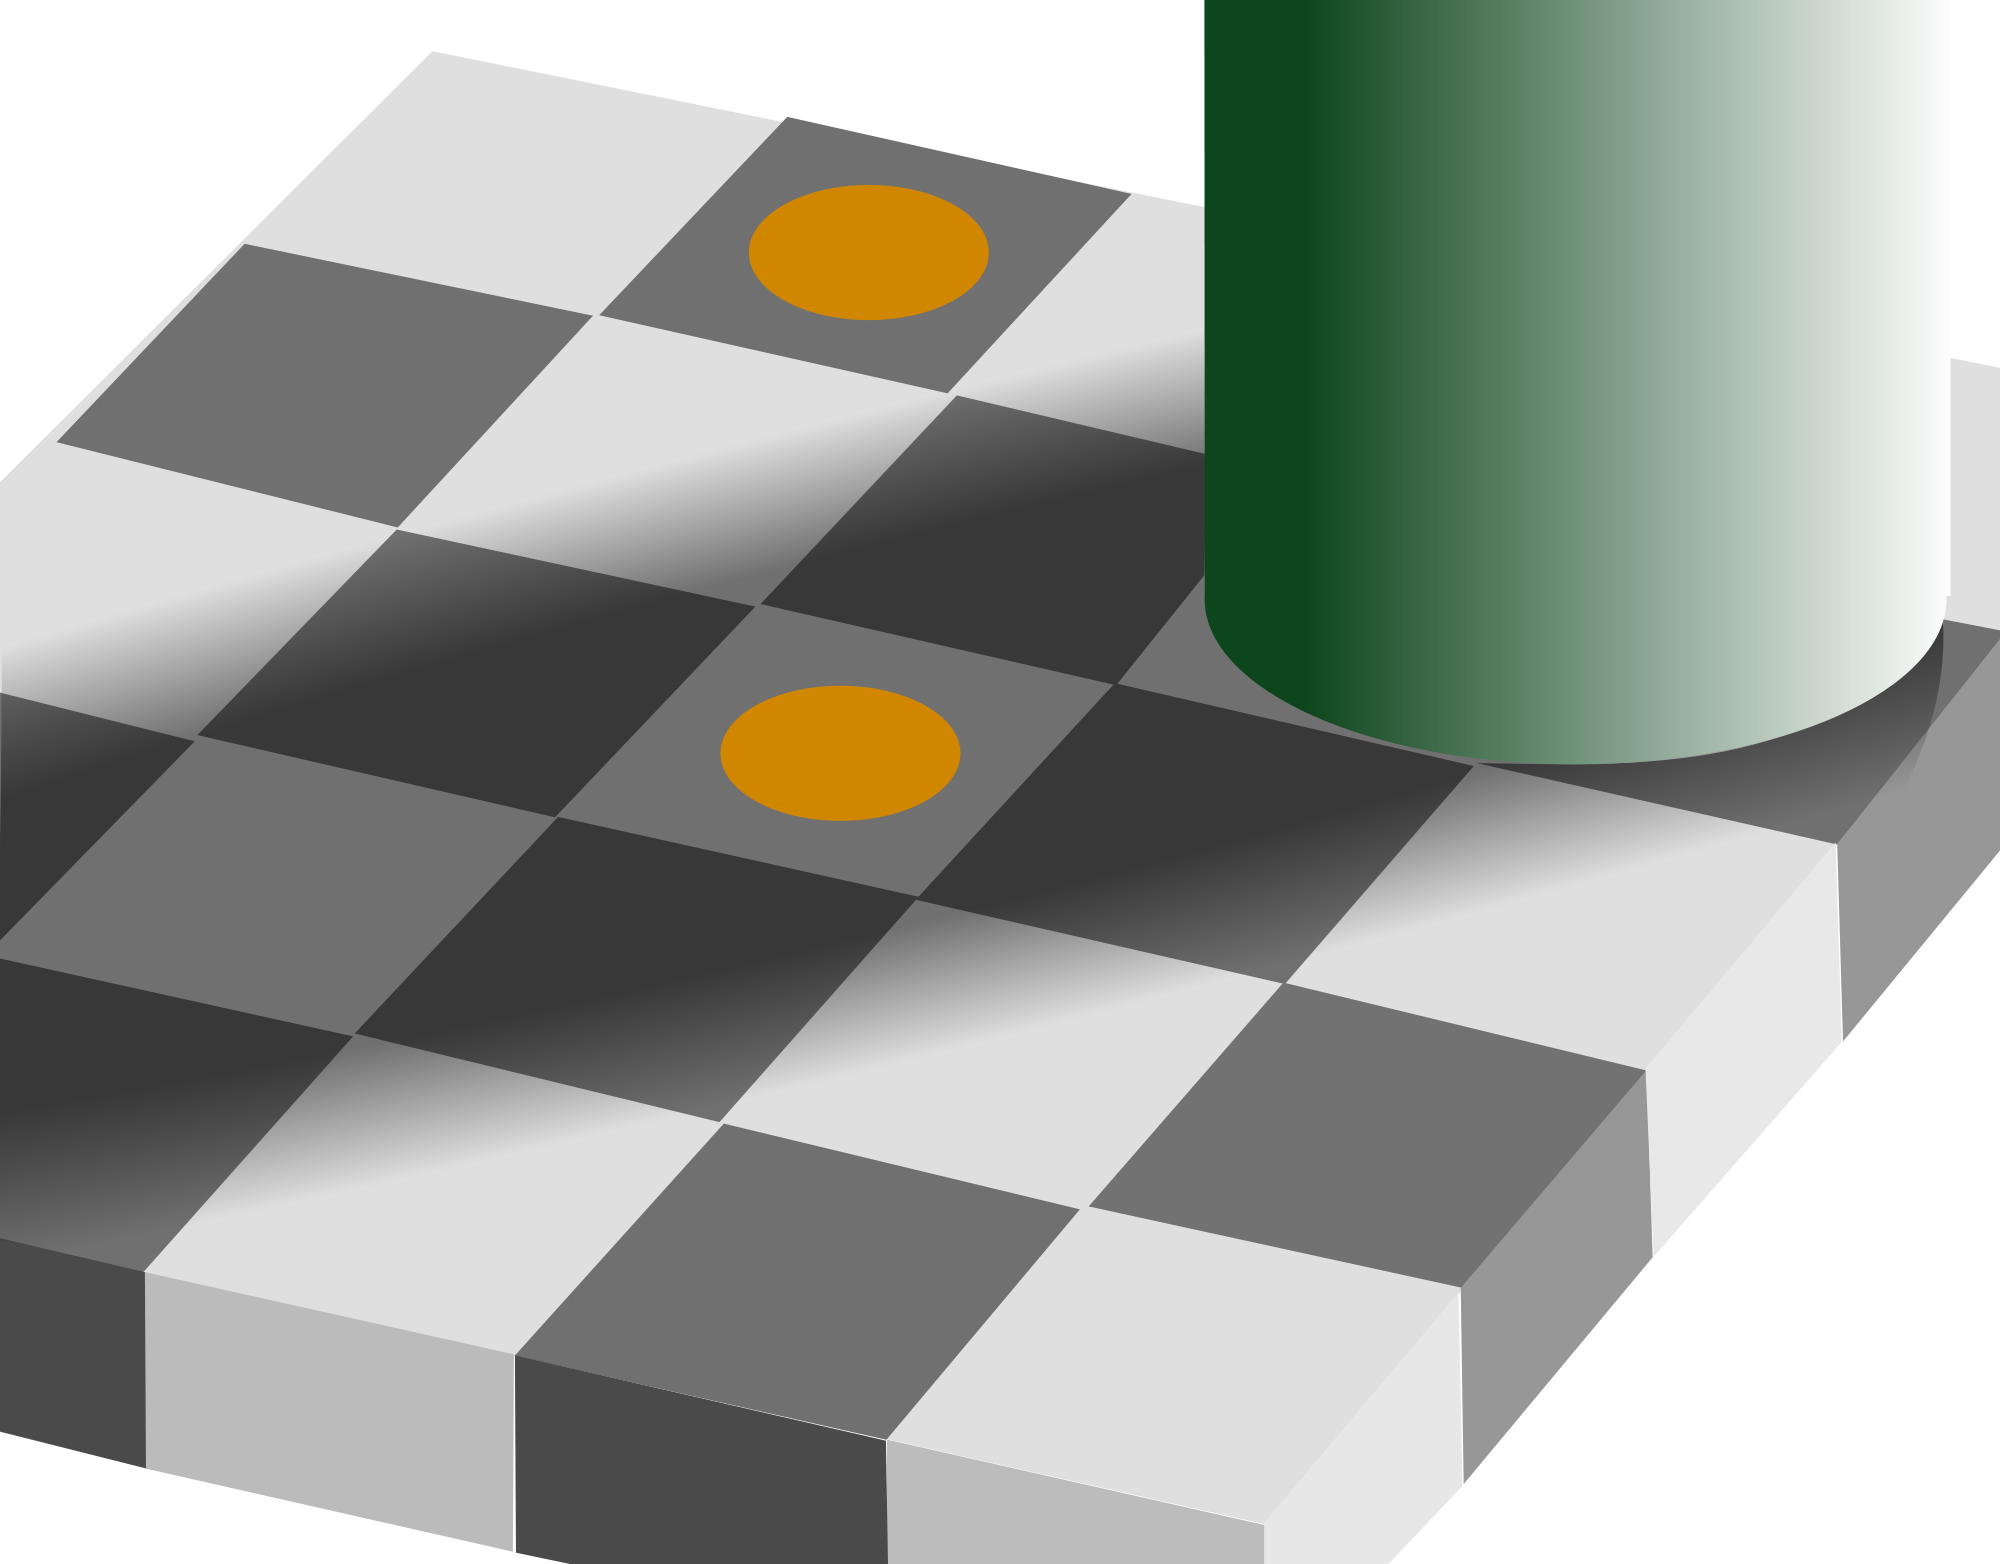
\includegraphics[width=50mm,height=50mm]{image01.png}
	\end{figure}
	
When it comes to faces there are two main ways illumination could degrade our images.  One, a uniform change in ambient 
light.  This occurs when the light source is straight on, visually the whole image gets darker or brighter.  Two, 
localised lighting changes, e.g. the light source is to the right of the face, so the left side is darker than the right.  
This is a distinction we will come back to later.  Illumination is clearly something any face recognition service will 
have to take into account if it wishes to accurately recognize a set of faces.  Thus, illumination is a logical and 
readily available normalization target to test the ease of use of my system.

\section{Comparing Two Methods}
The plan will be to test a newly proposed method of illumination correction, The Mean Illumination Estimation (MIE) 
~\cite{LuoaRINMBoMEfFR}, against something with proven results, namely, OpenCV's built-in histogram equalization.  We 
have the proposition put forward by ~\cite{LuoaRINMBoMEfFR} that their algorithm bests the current standard for 
illumination correction.  This implies that it should fare better than a simple quick and easy Histogram Equalization 
technique from OpenCV.

\subsection{Histogram Equalization}
As stated we will be employing OpenCV's implementation of this algorithm.  However, presented below is an overview on 
how the algorithm works and why it is theoretically useful to correct for different illumination conditions. \\

\pagebreak

Before we get into the math of the method an intuitive description would be useful.  Ideally what would happen using histogram 
equalization is given an image with 256 pixels and applying histogram equalization, one pixel will have a value of 1, another 
would have value 2, another would have value 255 etc.  Or if we had an image of 512 pixels, two would get a value of 0, another 
two would get 1 etc.  So a uniform distribution of pixel values is the goal.  However, doing so we would lose structure to our 
image as pixel values originally of the same intensity get mapped to different values ~\cite{urlIntuitiveHistEqualization}.  
So, at a minimum  we need to make sure that pixels of the same intensity value in the base image get transformed to the same 
``normalized'' intensity.  We also need to be careful that we don't affect the base structure of the image in another way i.e. 
pixel $(x_0, y_0)$ which is brighter than pixel $(x_1, y_1)$ put through this algorithm to get $(x'_0, y'_0)$ will still be 
brighter than $(x'_1, y'_1)$ though both values will likely have changed. \\

Mathematically we are mapping a clustered potentially non-uniform distribution to a wider (0-255) more uniform spread of 
intensity values.  Let $f$ be the given image represented by a $n \times m$ matrix of pixel intensities ranging from (0 to L-1) 
where $L$ is the number of possible values (usually 256) Now $p$ will denote the normalized histogram of our image $f$ as a list 
of bins per intensity value:

	\begin{equation}
		p_{n} = \frac{x_n}{Total} \quad n = 0,1,2,....,L-2, L-1
	\end{equation}
	
where $x_n$ is the number of pixels with intensity 'n' and 'Total' is the total number 
of pixels in the image.  We will define the Histogram equalized image as 'g';

	\begin{equation}
		g_{ij} = floor((L-1)\sum_{n=0}{f_{ij}} p_n )
	\end{equation}
	
Note floor rounds down the value.  The explanation used here can be found from the University of California 
~\cite{urlHistEqualization}

\subsection{Summary of Histogram Equalization}
Now we have a normalised image with which we can hopefully perform recognition on with greater success.  We note that technically 
it doesn't really care that there are illumination issues present.  Histogram equalization is a global image operation that will 
effect the entire image in the same way, regardless of the actual lighting conditions present in portions of the image.  i.e. if we 
took a face image with one half bright and one half dark and put it through the algorithm, as already stated above, the brighter 
pixels on the one half will still be brighter after the equalization is performed which still equates to an illumination problem 
for the Eigenface algorithm.  However, these are very much edge cases.  For the most part illumination issues will be of the form 
of global lighting differences.


\subsection{Mean Illumination Estimation}
	This method takes a localised smoothing approach to lighting normalization.  This is done so as to remove the components of 
	the image responsible for illumination changes.  Firstly it notes that according to the Illumination-Reflection model described 
	in detail in ~\cite{JianSaCSiIaSRCTaA}, a pixel $f_{xy}$ in a facial image gets its value from two components. $r_{xy}$ 
	represents the reflection component of an image at the point $(x,y)$ and $i_{xy}$ represents the illumination component.  Thus 
	we get the equation:
		
		\begin{equation}
			f_{xy} = r_{xy}	\times i_{xy}	
		\end{equation}
		
	Now, as $r_{xy}$ is dependant purely on the surface material in question and not affected by illumination it would be an 
	intrinsic representation of the facial image.  Suppose $i_{xy}$ changes little in value	within a small area while in the 
	presence of a weak light source.  The key idea now is to estimate the regional value of the illumination and use this to 
	cancel out the illumination. Thus we wish to find an estimate of our image $f_{xy}$ that will allow us to do this separation.  
	To attain such an estimate we apply a logarithmic transformation to each pixel in our image $f_{xy}$ we call this new function 
	$g_{xy}$
		
		\begin{align}
			g_{xy} &= ln(f_{xy}) \nonumber \\
			&= ln(r_{xy}) + ln(i_{xy})
		\end{align}
		
	Now $\hat{g}_{xy}$ becomes a mean estimate for $g_{xy}$ and is obtained via: 
		
		\begin{align}
			\hat{g}_{xy} &= \frac{1}{n^2} \sum_{(s,t)\in\omega_{nn}} g_{st} \nonumber \\
			&=  \frac{1}{n^2} \sum_{(s,t)\in\omega_{nn}} ln(r_{st}) + \frac{1}{n^2} \sum_{(s,t)\in\omega_{nn}} ln(i_{st})
		\end{align}

	Note $\omega_{nn}$ is the area around a given pixel $(x,y)$ with $(s,t)$ being the enumeration of these pixels and n is the 
	width/height of said kernel around $(x,y)$.  Next, the quotient image $d_{xy}$ is constructed from equations, (2.4),(2.5) we 
	do so to eliminate $i_{xy}$ (or make its contribution to the image negligible):
		
		\begin{align}
			d_{xy} &= g_{xy} - \hat{g}_{xy} 	\nonumber \\
			&= ln(r_{xy}) - \frac{1}{n^2} \sum_{(s,t)\in\omega_{nn}} ln(r_{xy}) + \sigma
		\end{align} 
		
	Where: $\sigma = ln(i_{xy}) -(\frac{1}{n^2})\sum_{(s,t)\in\omega_{nn}} ln(i_{st})$ we note that $\sigma$ will be a very small 
	value and can hence be omitted from (4) leaving us with the relation:
		
		\begin{align}
		d_{xy} &= g_{xy} - \hat{g}_{xy} \nonumber \\
		&\approx ln(\frac{r_{xy}}{(\prod_{(s,t)\in\omega_{nn}} r_{st})^{\frac{1}{\pi^2}} })
		\end{align}
		
	Now, $d_{xy}$ represents the ratio between the current point's reflectance and the average reflectance around it.  When the 
	materials in the localised kernel around (x,y) are the same $d_{xy}$ tends towards zero, but when they are different e.g. 
	facial skin and facial features $d_{xy}$ becomes notably none-zero.  Let us consider:
		
		\begin{equation}
			\alpha = \frac{1}{ab}\sum_{(x,y)\in f_{a \times b}} |d_{xy}| 
		\end{equation}
		
	With $a$ = number of rows and $b$ = number of columns in an image $f_{a \times b}$.  $\alpha$ will represent the average grey 
	value ratio of the whole image and features.  Each pixel is hence expressed as the ratio exponent relative to the average grey 
	value:
		
		\begin{equation}
			h_{xy} = \exp{\frac{d_{xy}}{\alpha \dot \beta}}
		\end{equation}
		
	With $\beta$ being a controllable scaling factor.  However, it is usually set in the range of two to three.  Finally to improve 
	contrast and correct the resulting brightness level, highlight facial features and reduce impact of background noise, post 
	processing is done as:
		
		\begin{equation}
			\hat{o}_{xy} = \left\{
				\begin{array}{l l}
					h_{xy} 	& \quad h_{xy} < 1 \\
					1 		& \quad h_{xy} \geq 1
				\end{array} \right.
		\end{equation}
		\begin{equation}
			o_{xy} = [\frac{255 \times (\hat{o}_{xy} -c)}{1-c}]
		\end{equation}
		
	With $o_{xy}$ being the final result image to be used in training or recognition.  $c$ is the minimum value of $\hat{o}_{xy}$.  
	The math may be complex but the idea is rather simple, given an image, we separate out the intensity factor from the structure 
	of the face, setting it to zero and rebuilding the face.  An example is provided below. 
	
		\begin{figure}[h!]
			\centering
			\caption{Mean Illumination Estimation images before and after applying MIE taken from~\cite{LuoaRINMBoMEfFR}\label{fig:MIE}}
			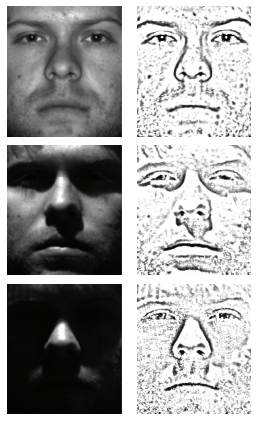
\includegraphics[width=75mm,height=120mm]{MIE.png}
		\end{figure}

	Notice here that the lighting angles have changed.  In the first image, the ambient light is full-frontal whereas the remaining 
	two images show shadows cast from various facial features ie directional lighting is present from this we gather the middle image 
	to be lit from about a 10'o'clock angle and the bottom image to be solely lit from above. \\
			
	The MIE algorithm leaves us with an image that for the most part is devoid of all extra light.  Ideally, multiple images of the same object 
	under different lighting conditions that are put through this algorithm will end up looking the same.  An example of it in use 
	can be seen below.  Note how, in the above fig:[~\ref{fig:MIE}], despite the drastic differences in illumination on the before 
	images, the right side varies little from face to face. \\
		
	The above images were 168x192 in size and it was discovered that for this size an n of 11 was optimal along with $\beta = 2.2$ 
	where $\beta$ is affected by facial reflectance of the subjects tested on.  However, it stays at a value of 2.2 as the facial 
	reflectance of different people varies little.
		
\subsection{Summary of Mean Illumination Estimation}
	The complications arise from estimating the illumination component so as to subtract it from the image, highlighting the remaining 
	reflectance of the image.  We achieve this by a logarithmic transform which only slightly (computationally) affects 
	the image, the fact remains that it still does change the image. \\
		
	In conclusion, any attempt to normalize an image's illumination will undoubtedly degrade some aspects of the image we would rather 
	retain.  However, one would hope that the gained standardization of facial images out way this degradation and yield more accurate 
	recognition rates.  We also note that this method is a localised correctional algorithm.  That is to say the afore mentioned issue 
	with histogram equalization not being very effective for images with half bright, half dark faces doesn't apply here.  The formula 
	and reasoning were put forward by and learned from ~\cite{LuoaRINMBoMEfFR}, an article that attempts to find a better way of solving 
	the lighting issue with positive results for their effort. \\
	
	Using the workstation, the task now is to gain more insight into the algorithm by attempting to duplicate the literature results 
	and to further validate the strengths and weaknesses of the algorithm.  The completed implementation of this algorithm in Python 
	can be seen in appendices:[A.1,A.2].  Note that little effort was made to optimise the program as the 
	implementation of the algorithm was a trial run to determine if the method would be useful for the system and our needs.  If the 
	algorithm does prove to be valuable, there are a number of means to improve efficiency as discussed at the end of the chapter.

\subsection{Validation of MIE implementation}
	Before the experiment can be run we first attempt to validate that aspects of the system work as intended.  
	This is done to provide validation to the results obtained from the experimental procedure.  Though we 
	predominantly wish to do so for our implementation of the Mean Illumination Estimation, for completion, we  
	also confirm OpenCV's built in Histogram Equalization method works as intended.

		\begin{figure}[H]
			\centering
			\caption{My MIE implementation [col 3] tested against provided example from ~\cite{LuoaRINMBoMEfFR} [col 2] \label{fig:MIE_Compariosn}}
			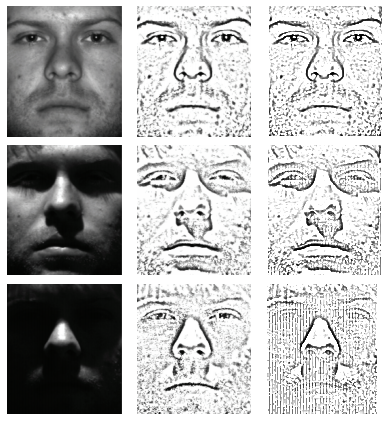
\includegraphics[width=75mm,height=80mm]{MIE_Compariosn.png}
		\end{figure}

	To start, we compare the output my MIE implementation provides against that of the output attained according 
	to ~\cite{LuoaRINMBoMEfFR}.  We note above in fig:[~\ref{fig:MIE_Compariosn}]; \\
	 
	We observe that my implementation provides near identical results to that of the article for the base face.  However, 
	as the images become darker our results seem to deviate more from those in the published paper.  We postulate that 
	these artefacts are being generated from the conversion between image to PDF used in the published paper, and back 
	to image again i.e. slight smudging and some significant frequency artefacts are introduced in the dark regions 
	from the conversion algorithm, possibly from compression algorithms. \\

	To confirm our hypothesis, here are several more images put through my algorithm that are not extracted from the PDF
	paper of ~\cite{LuoaRINMBoMEfFR}.  We see none of the below show similar artefacts to those found in 
	fig:[~\ref{fig:MIE_Compariosn}].

		\begin{figure}[H]
			\centering
			\caption{MIE implementation applied to CSC Honours 2015 Class list, Rhodes University. Some blacked out due to lack of permission from subjects\label{fig:MIE_training_data_from_my_method}}
			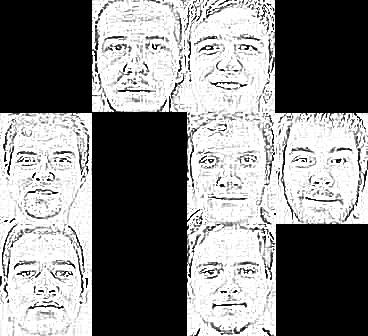
\includegraphics[width=120mm,height=115mm]{MIE_training_data_from_my_method.png}
		\end{figure}
	
	To further investigate, we took the original PDF images from the paper~\cite{LuoaRINMBoMEfFR} and ran them through the OpenCV implementation 
	of histogram equalization Below fig:[~\ref{fig:Hist_example}], we see the same faces as the MIE comparison test 
	fig:[~\ref{fig:MIE_Compariosn}] above.  However, instead of the MIE applied to them they have undergone histogram 
	equalization, an OpenCV algorithm in which there is a high confidence.

		\begin{figure}[H]
			\centering
			\caption{Histogram Equalization applied to article example faces~\cite{LuoaRINMBoMEfFR} \label{fig:Hist_example}}
			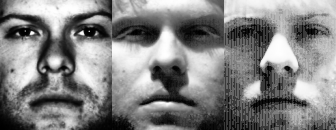
\includegraphics[width=100mm,height=40mm]{Hist_example.png}
		\end{figure}
		
	We see that the intensities have been stretched for all images, improving visibility, We also note in the middle 
	image around the eyes and in the far right image, once again the same artefact pattern emerges.  This points again 
	to an issue with the image itself, not the algorithms performed upon them.  \\
	
	Now that we have built confidence in our implemented code that it does work as intended by the original creators 
	we can construct an experiment to test the effects on accuracy they have.
	
\section{Reading The Graphs}
The algorithm ``classifies'' a face provided the matcher gets a ``deviation'' score less than the provided threshold.   Therefore 
at each threshold point we get three regions; going up; the first region defines the number of successfully classified images, 
the second region shows the number of unsuccessful classifications and the remaining portion of the graph are those images that 
were not yet classified under the current threshold but may still be under the next threshold level. 

\newpage
\section{A word on training}
We train the eigenface method with multiple images per subject.  This is done to increase accuracy of the system.  Having 
multiple images of the same person under different conditions provides a higher likelihood for the system to correctly match 
a new face to one of the subjects training data.  E.g. we train with 10 subjects, each subject has 5 training images one 
looking up, down, left, right and full-frontal we label each image as subject 1.  Thus, given a new image of the subject 
looking left, there is a higher probability for a successful match to subject 1 as the system has a training image of that 
subject looking left.

\section{Experiment 01: Setup}
First up we will test our system against the AT\&T database, this database contains 40 subjects with 10 images per subject 
totalling 400 images~\cite{ATTDATA}.  We have evenly split this data into training and test data i.e. 5 images per subject goes to 
training and the other five to test data.   The results we will be comparing are the total number of correct connections 
made by the Eigenface algorithm.  This database primarily focuses on orientation of the subjects faces and has limited 
illumination variance, as such, we expect the Eigenface algorithm to perform with some degree of accuracy and the application 
of our two normalisation techniques to have minimal if any effect on the accuracies obtained. 

\subsection{Experiment 01: Results}
We start with a base line, no normalization techniques used, just the plain dataset run through the 
Eigenface algorithm.  Doing so we get the graph;

	\begin{figure}[H]
		\centering
		\caption{Base line, no illumination normalization used; AT\&T \label{fig:Att_BaseLine}}
		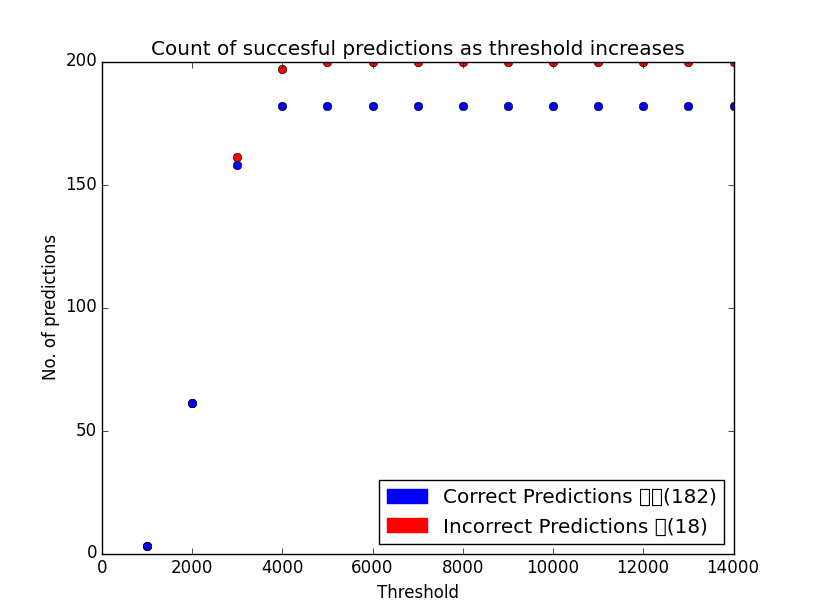
\includegraphics[width=100mm,height=70mm]{Att_full_None.png}
	\end{figure}

From Figure:~\ref{fig:Att_BaseLine} we see that we correctly recognize $\frac{182}{200}$ subject images i.e. equating to a 
91\% accuracy.  We run the experiment again but this time perform histogram equalization upon both test and training data.  
This provides us with the graph; 

	\begin{figure}[H]
		\centering
		\caption{Histogram Equalization experiment; AT\&T \label{fig:Att_Hist_exp}}
		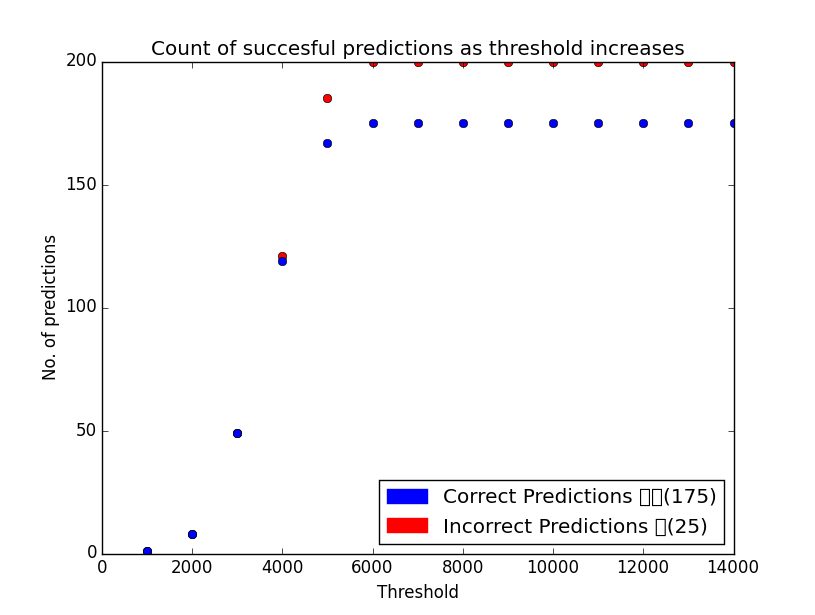
\includegraphics[width=100mm,height=70mm]{Att_full_Hist.png}
	\end{figure}
	
We now see from Figure:~\ref{fig:Att_Hist_exp} that the system can correctly recognize $\frac{175}{200}$ of the subject images,
roughly 87\% accuracy rating, a slight drop from the base line but still a viable accuracy.  we also note that it is significant 
that at lower threshold values, almost no incorrect classifications are made.  As we increase the threshold after about 80\% 
correctly classified, the final 20\% have about an equal number of correct and incorrect classifications occur.  
We now run the experiment again.  However, now we test our MIE algorithm.  Doing so, we obtain the results;

	\begin{figure}[H]
		\centering
		\caption{MIE experiment; AT\&T \label{fig:Att_MIE_exp}}
		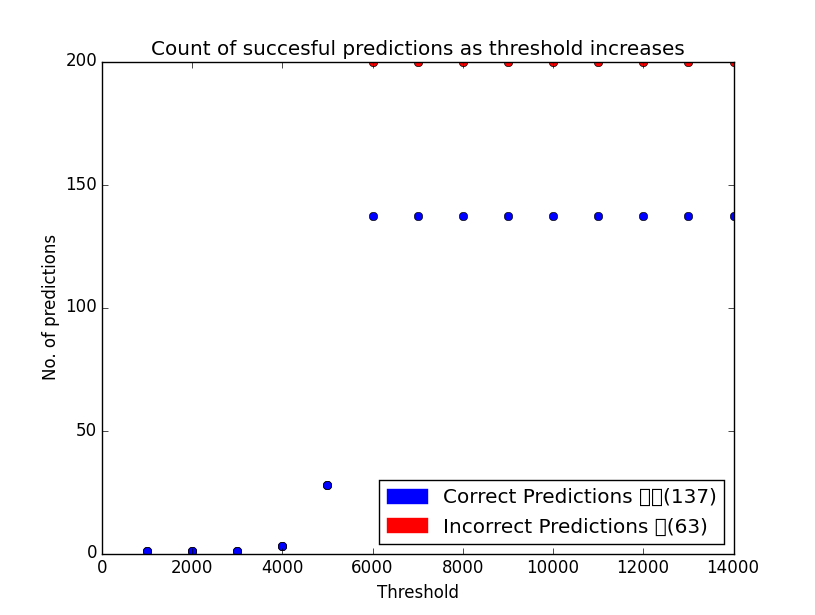
\includegraphics[width=100mm,height=70mm]{Att_full_MIE.png}
	\end{figure}

Here we see greatly diminished results with, $\frac{137}{200}$ recognized faces, equating to roughly 68\% accuracy.  Once again, 
we try two more experiments, 1.) we run histogram equalization first, then MIE upon this normalised data. 2.) the other way round, 
test MIE first, then histogram equalization;
 
 	\begin{figure}[H]
		\centering
		\caption{Histogram then MIE; AT\&T \label{fig:Att_Hist_MIE_exp}}
		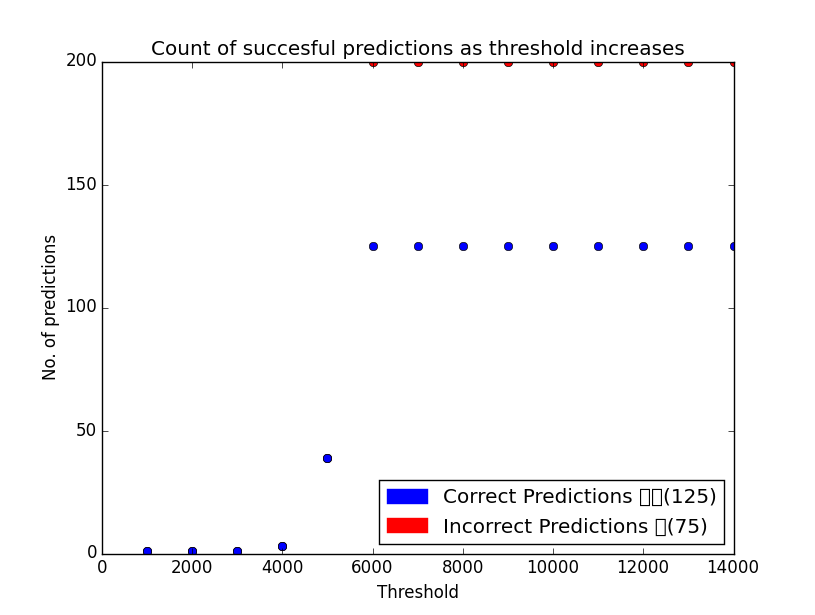
\includegraphics[width=100mm,height=70mm]{Att_full_Hist_MIE.png}
	\end{figure}
	
   	\begin{figure}[H]
		\centering
		\caption{MIE then Histogram; AT\&T \label{fig:Att_MIE_Hist_exp}}
		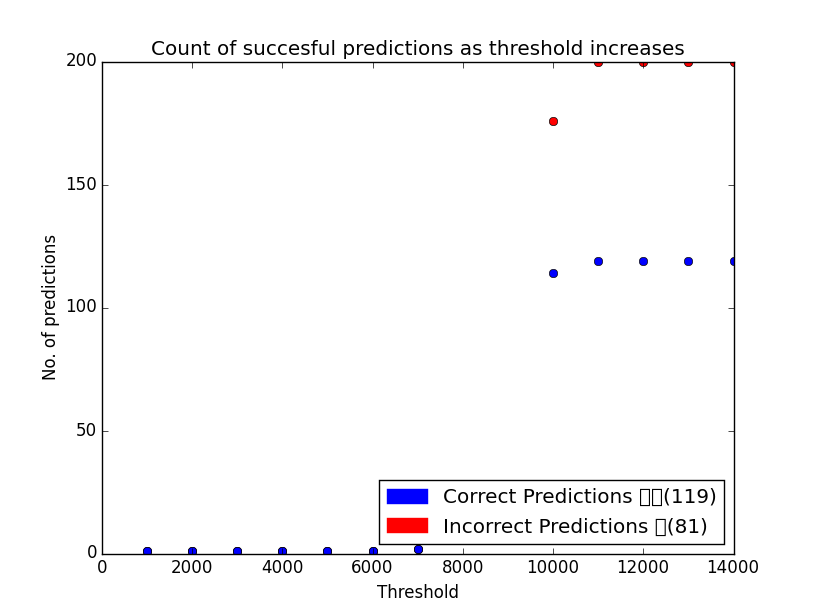
\includegraphics[width=100mm,height=70mm]{Att_full_MIE_Hist.png}
	\end{figure}
  
Aside from the over all inaccuracy of the combination we see a connection emerge; histogram equalization then MIE performs 
in accordance with MIE on its own if slightly less accurate but the other way round provides far worse results.

\subsection{Experiment 01: Discussion}
Initially we observed what we expected, the baseline performed with a high degree of accuracy due to the lack of illumination 
change in the images.  However, to our disappointment when we run our correction algorithms we see diminished results with 
MIE being completely impractical for normal use.  \\

\section{Experiment 02: Setup}
For this experiment the conditions were; Yale B face database ~\cite{KCLee05} which contains 38 individuals with 65 images per 
subject (2470 total).  However, to reduce computation time I will only used a subset of the data, the first 20 subjects. Note, 
the Eigenface algorithm cannot handle images of varying size,  so many of the subjects have images that need to be discarded as 
they are larger than the others panned out larger and needing to be cropped.  Also, some of the images were provided as corrupt, 
presumably as further testing data, they too have been removed.  Furthermore we also take 10 images per subject to use as the 
training set.  What remains is 20 subjects and 1072 images as testing data.  The results we will be comparing are the total number 
of correct connections made by the Eigenface algorithm.  Based on the literature and as noted above, we expect MIE to surpass 
OpenCV's Histogram equalizations recognition accuracy.

\subsection{Experiment 02: Results}
As before we start with a base line, no normalization techniques used, just the plain dataset run through the 
Eigenface algorithm.  Doing so we get the graph:

	\begin{figure}[H]
		\centering
		\caption{Base line, no illumination normalization used; Yale B\label{fig:BaseLine}}
		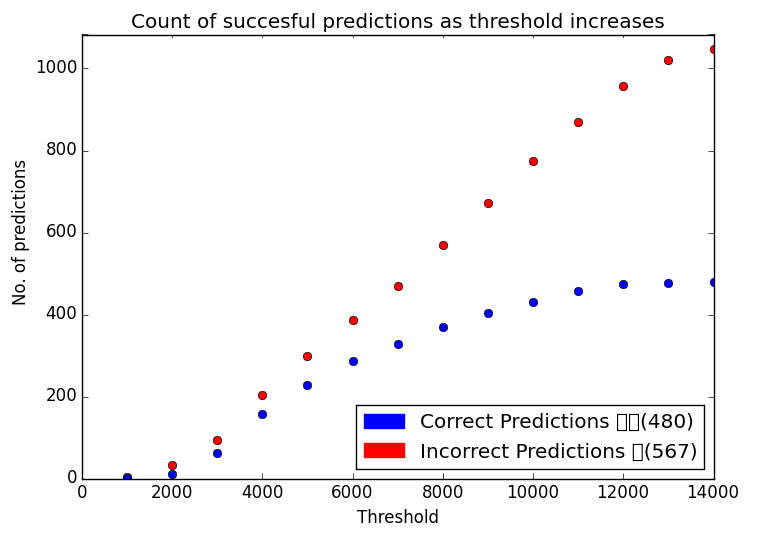
\includegraphics[width=100mm,height=70mm]{Yale_half_None.png}
	\end{figure}
By contrast to the previous dataset, here we see incorrect classifications even at low threshold values and a flat-lining of 
the correct predictions graph i.e. increasing the threshold will give more inaccurate classifications then correct ones.
From fig:[~\ref{fig:BaseLine}] we see that we correctly recognize $\frac{480}{1072}$ subject images i.e. roughly 45\% 
accuracy.  We run the experiment again but this time perform histogram equalization upon both test and training data.  
This provides us with the graph; 

	\begin{figure}[H]
		\centering
		\caption{Histogram equalization experiment; Yale B \label{fig:Hist_exp}}
		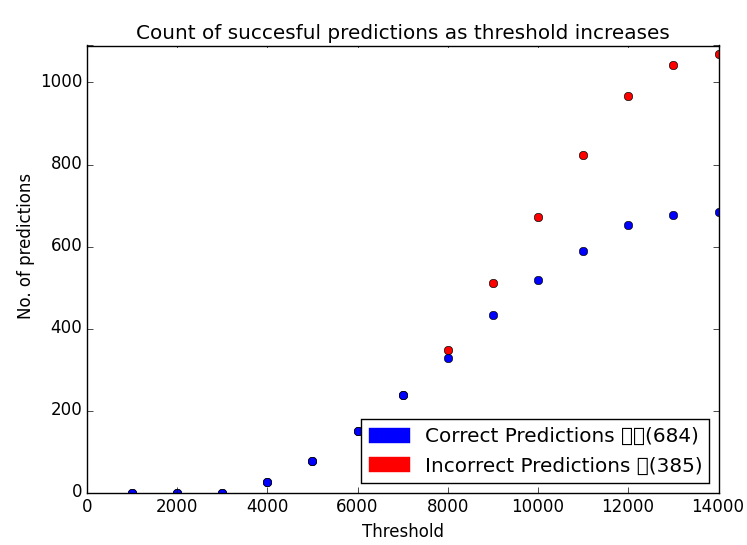
\includegraphics[width=100mm,height=70mm]{Yale_half_Hist.png}
	\end{figure}
	
We now see from fig:~\ref{fig:Hist_exp} that the system can correctly recognize $\frac{684}{1072}$ of the subject images, 
roughly 64\% accuracy rating, a meaningful improvement on the base line.  \\

We now run the experiment again.  However, instead of Histogram Equalization, we test our MIE algorithm.  Doing so, we obtain 
the results.

	\begin{figure}[H]
		\centering
		\caption{MIE experiment; Yale B \label{fig:MIE_exp}}
		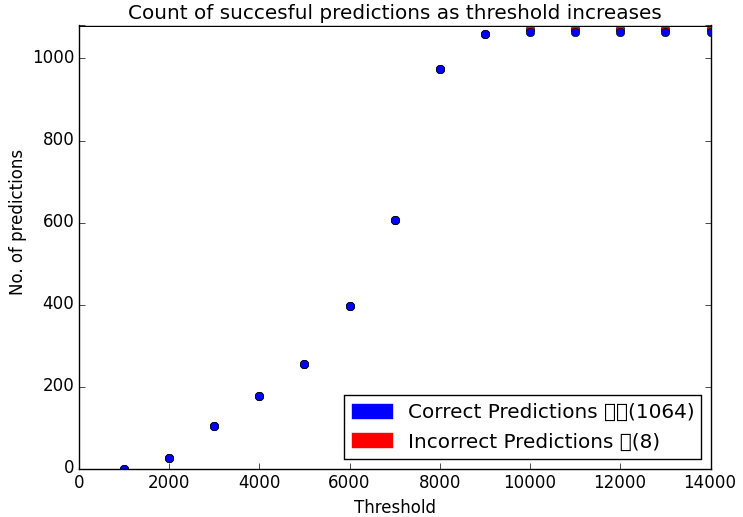
\includegraphics[width=100mm,height=70mm]{Yale_half_MIE.png}
	\end{figure}

Here we see greatly improved results with, $\frac{1064}{1072}$ recognized faces, 
equating to roughly 99\% accuracy. \\ 

In a final attempt to yield even better results, we performed two more experiments, 1.) we run histogram equalization first, 
then MIE upon this normalised data. 2.) the other way round, apply MIE first, then apply histogram equalization.
 
 	\begin{figure}[H]
		\centering
		\caption{Histogram then MIE; Yale B \label{fig:Hist_MIE_exp}}
		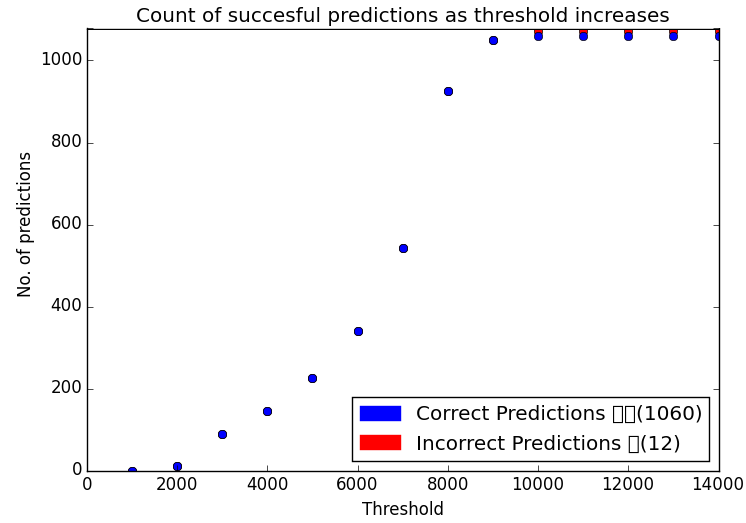
\includegraphics[width=100mm,height=70mm]{Yale_half_Hist_MIE.png}
	\end{figure}
	
   	\begin{figure}[H]
		\centering
		\caption{MIE then Histogram; Yale B \label{fig:MIE_Hist_exp}}
		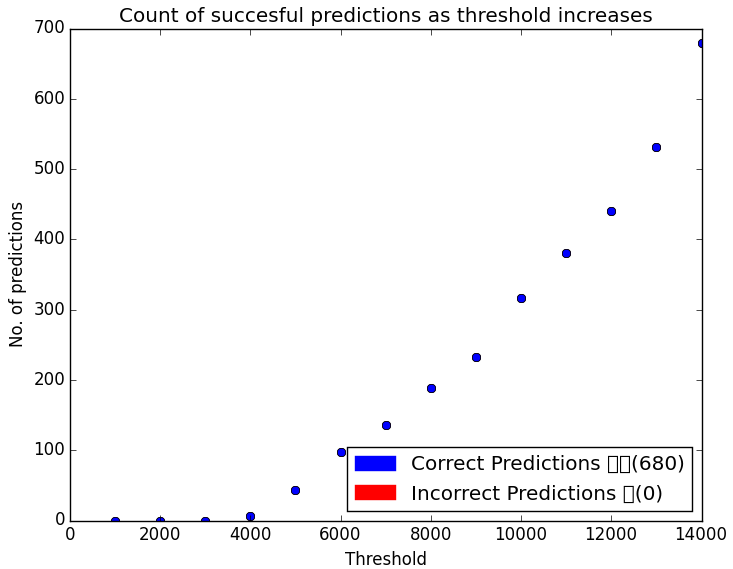
\includegraphics[width=100mm,height=70mm]{Yale_half_MIE_Hist.png}
	\end{figure}
  
We see from these experiments that Performing Histogram Equalization first and then MIE on top of that performs nearly as 
well as MIE on its own, but the other way round yields shocking results, failing to even score all images under the maximum 
14000 threshold.  It is significant though, that this combination makes very few misclassification (None, in fact, in fig:~\ref{fig:MIE_Hist_exp})

\subsection{Experiment 02: Discussion}
The Baseline experiment, fig:[~\ref{fig:BaseLine}] provides a very poor score with this facial database, this was to be 
expected due to the high impact of lighting conditions on the Eigenface algorithm, yielding a score of $\frac{480}{1072}$, 
roughly 45\% accuracy.  On top of that, it technically doesn't even score all the images, 3 were missed i.e. their threshold 
values were higher than the upper limit of our graph. \\

The first experiment we try is histogram equalization.  Here we see an improvement in recognition at roughly 64\%.  We 
already know from the explanation of the workings of histogram equalization that it is not ideal for the Eigenface
method when used on images with localised lighting conditions, something that the Yale B database has in abundance.  
This aside, all in all, it is a notable improvement on the none-normalised score but still far from the ideal. \\

Next we hope to achieve better results with the MIE version of the data.  We get results which far surpass those provided 
by histogram equalization, at roughly 99\%. This is because the MIE is a very localised oriented algorithm and as the Yale B 
database has nearly insignificant change in orientation and angle, purely lighting changes, the MIE performs well.  
As such, these results most certainly agree with the claim published in~\cite{LuoaRINMBoMEfFR}. \\

With regards to the compound tests I deduce the reason for such discrepancy between the order is that performing histogram 
equalization first outputs a very lightly affected image with just a simple contrast change that MIE can operate on in much 
the same way as before, while trying to do it the other way, MIE outputs a vastly different image from the original, more 
resembling a sketch than a photo, with large variation in colour intensities,  as such the histogram equalization algorithm 
falters as we have reduced the colour space to an even more compact region of the spectrum.  Thus when we pass these new 
images through the histogram equalization method it just does more damage by stretching it further.  \\

What we take away from this is that although MIE performs phenomenally against strong illumination conditions it tends to 
degrade the image it is working on to an extent that other normalization techniques are ineffective at best and further 
degrading at worst. \\

In reality we probably wouldn't want to perform multiple normalization techniques that target the same issue upon our dataset 
as we would expect such conflicts to arise.  On the other hand we would hope that combining these techniques with others that 
target different aspects of normalization would not conflict with each other.  Indeed, we would hope that doing so would provide
a higher degree of accuracy in recognition.


\section{Summary}
This chapter confirms the claim made earlier that the Eigenface algorithm is very sensitive to lighting fig:[~\ref{fig:BaseLine}]
showed very low recognition rates, yet the same data improved spectacularly after MIE was applied fig:[~\ref{fig:MIE_exp}] \\

To conclude, yes, MIE looks good, but only for a narrow category of normalization problems namely, those with localized regions of 
lighting variation on that note, I find it hard to believe any algorithm could improve upon those accuracies.  Sadly that's where the 
downsides must be mentioned.  The algorithm doesn't play well with other techniques and even less so when there are no local 
illumination issues present, tending to be more of a hindrance than a help.  Taking note of this, for our implementation in classroom 
attendance tracking, we have a semi-controlled environment where lighting conditions will be more along the lines of uniform 
differences across our subject faces.  As such OpenCV's histogram equalization would be the algorithm of choice for our needs.  \\

The very low rate of miscalculations using the combined algorithms might have uses elsewhere.  In some scenarios a ``false classification'' 
might be very costly - i.e. In airport security, it would require pulling the individual from the queue for further interrogation. \\

The Python implementation of MIE was horribly time inefficient.  As a benchmark, OpenCV's histogram equalisation was performed 
upon the 1272 images and did so in under a minute while my Python implementation of MIE took roughly 10hrs to do the same number of images. 
Again, this speed difference comes with the benefit of being a very localised method.  Each pixel is compared to a 11x11 kernel 
around itself as well as the average intensity for the whole image.  This means it can handle images which are dark on one side but 
light on the other without problems. \\  

It was beyond the scope of this work to attempt to optimise this method. However, we do note the following possible optimisations; \\
1.) Converting the MIE code logic into C++ or C that is then wrapped into Python, doing so could offer substantial speed-ups. \\
2.) The current implementation is fairly naive: the 11x11 region is recomputed for each pixel in the image.  Many efficient image 
processing algorithms operate by sliding a difference window over the image and computing a running estimate of local intensity in 
our case we would reduce the 121 computations to 22 per pixel.  This would most certainly improve the performance of the method. 
Finally, this per pixel kernel methodology indicates that this method could see a large speed-up if performed through a GPU.  
However, these are ideas for future work to look into.



